\subsubsection{Conflict} \label{odp_conflict}
% Subsection structure:
% Problem: what is the generalized problem?
% 	Motivation: why is this problem scientifically important and/or interesting?
% Solution: conceptual description of solution, including formal definition of GODP and SHACL shapes.
% 	Illustration: images of GODP structure.
% 	(Statistical)Analysis: how does the solution solve the problem?
% 	Evaluation: are the results significant? What is the impact?
\paragraph{Detecting conflict}
Information that has conflicting evidence sources is less reliable compared to information that does not have conflicting evidence sources. For example, stakeholder experience that is conflicting with evaluated external evidence is less reliable compared to stakeholder experience that does not have any conflict. We define the number of evidence sources that causes a conflict with the decision-relevant information as the level of conflict. We define the level of conflict using the reproducibility of information. When information is reproducible by one evidence source, and this evidence source has one additional conflicting evidence source, the level of conflict is $1$. When the evidence source has two conflicting evidence sources, the level of conflict is $2$. Compared to a fuzzy approach that can classify certain conflict levels as, for example, $low$, $medium$, or $high$, the number-based approach makes it easier to compare conflict levels. We do not compare conflict-levels in this study.

\begin{center}
\large\color{document}{The conflict pattern validates information reliability by detecting conflicting evidence.} 
\end{center}

\paragraph{Ontology}
We define conflicting evidence as evidence that disagrees with another evidence source. The reproducibility pattern serves as a natural base for the conflict pattern. The reproducibility pattern provides the structure on which we create the conflict pattern using the object property $disagrees\_with$. Figure \ref{fig:conflict} presents the conflict pattern. We mark the extension of the conflict pattern in \textcolor{Red}{red}. We measure the level of conflict between evidence sources using the $disagrees\_with$ object property. For example, if two stakeholders have a different experience, the $disagrees\_with$ object property represents this conflicting stakeholder experience. 

\begin{figure}[H]
\centering
  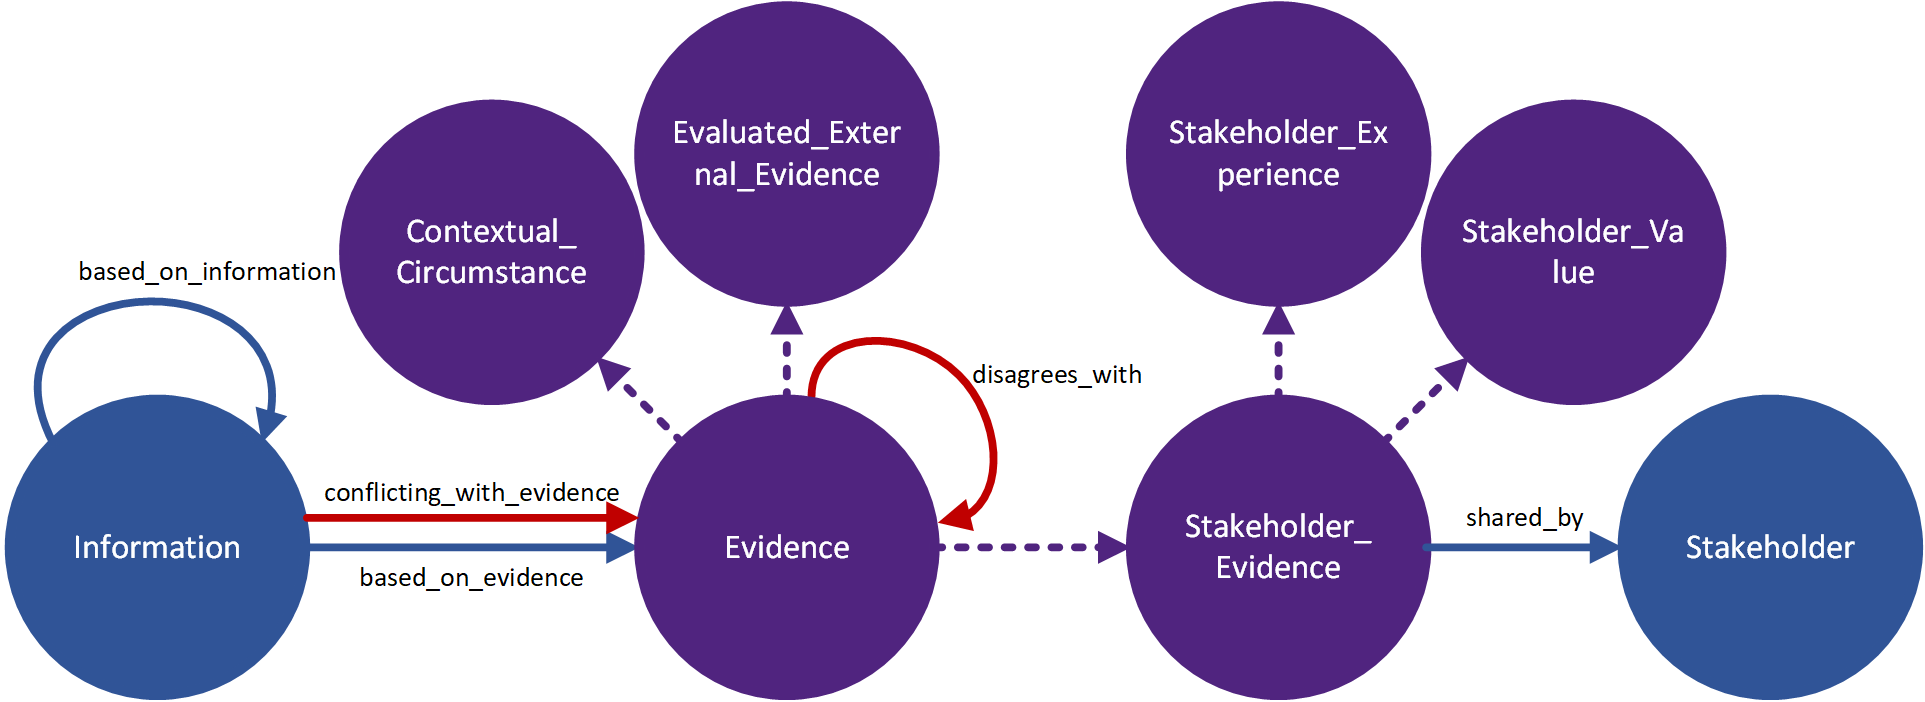
\includegraphics[width=14cm]{../../Images/04_Contribution/04_Conflict_Ontology.png}
  \caption{The conflict pattern uses the reproducibility pattern and extends it with the object property $disagrees\_with$. Code sample \ref{GODP_CONF_LEV} presents the GDOL code for instantiating the conflict pattern.}
  \label{fig:conflict}
\end{figure}

\paragraph{Inferencing}
We introduce an additional object property: $conflict\_with\_evidence$. When we base $In{\f}ormationX$ on $EvidenceA$, and $EvidenceA$ disagrees with $EvidenceB$, $In{\f}ormationX$ conflicts with $EvidenceB$. This conflict reduces trust in $In{\f}ormationX$. Figure \ref{fig:conflict_inferred} presents the super property that infers this knowledge from the existing ontology structure.

\begin{figure}[H]
\centering
  
\includegraphics[width=17cm]{../../Images/Conflict_Inferred.png}
  \caption{The configuration of the super property that infers the object property $conflict\_with\_evidence$ in Prot\'eg\'e.}
  \label{fig:conflict_inferred}
\end{figure}

$disagrees\_with$ is symmetric and irreflexive. Disagreement is always symmetric: if $StakeholderA$ disagrees with $StakeholderB$ on a specific subject, then $StakeholderB$ also disagrees with $StakeholderA$. Figure \ref{fig:conflict_irreflexive} presents the situation in which $disagrees\_with$ is symmetric and irreflexive.

\begin{figure}[H]
\centering
  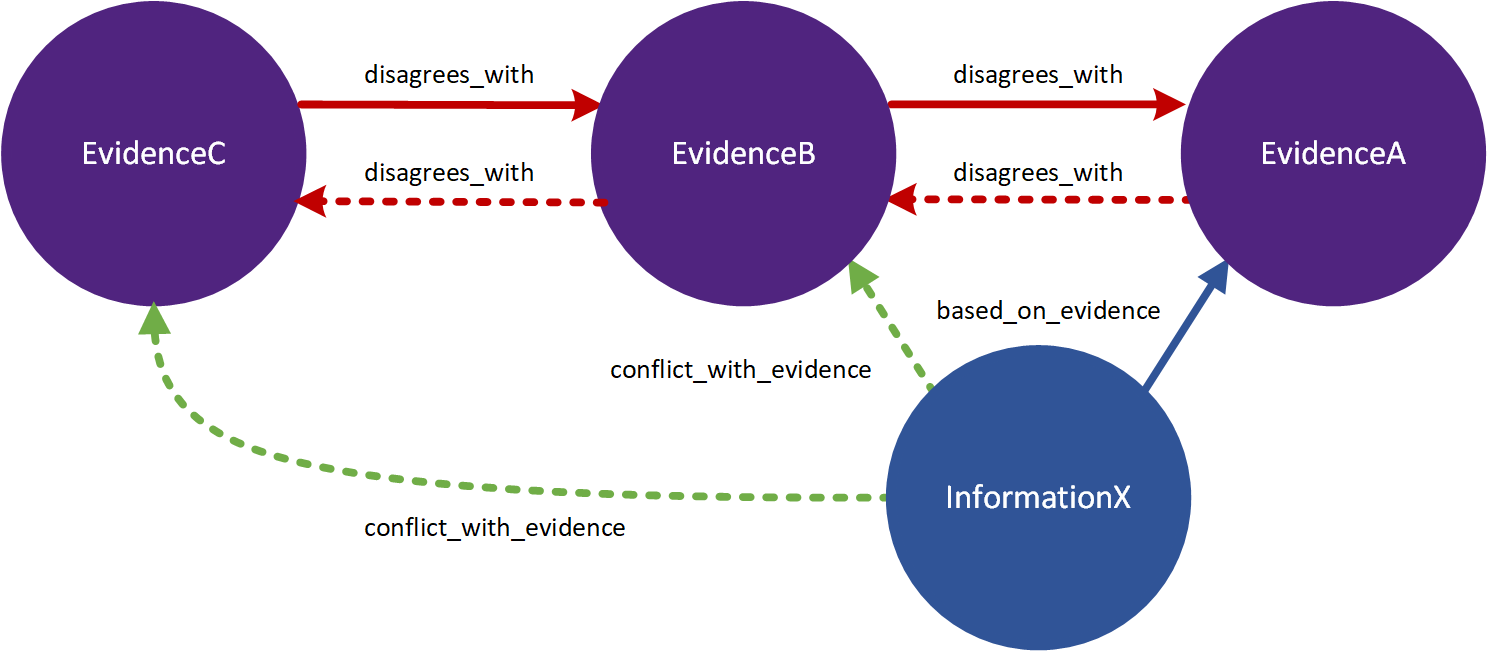
\includegraphics[width=13cm]{../../Images/04_Contribution/04_Conflict_Characteristics.png}
  \caption{The symmetric and irreflexive characteristics of $disagrees\_with$. The reasoner infers the dotted lines based on the super property figure \ref{fig:conflict_inferred} presents.}
  \label{fig:conflict_irreflexive}
\end{figure}

\paragraph{Inconsistency}
The consensus pattern inherits the consistency validation from the reproducibility pattern. We describe the consistency of the reproducibility pattern in section \ref{rep_incons} \nameref{rep_incons}.

Figure \ref{fig:conflict_transitive} presents the hypothetical situation in which $disagrees\_with$ is symmetric, transitive, and irreflexive. This situation results in an inconsistent ontology. The reasoner infers the $disagrees\_with$ object property on $EvidenceA$ based on the transitivity characteristic. This object property causes conflict with the irreflexive character of $disagrees\_with$. The transitivity helps us to discover disagreement chains and ensures we present the right conflict level to the decision-maker. Transitivity causes a problem: evidence cannot disagree with itself. When we combine the irreflexive and transitive characteristics, the reasoner might infer the $disagrees\_with$ object property on an evidence source. For example, we assume $R$ is transitive and irreflexive. By transitivity, we conclude $xRy \land yRx \rightarrow xRx$. However, this is not possible as $R$ should be irreflexive as well.

\begin{figure}[H]
\centering
  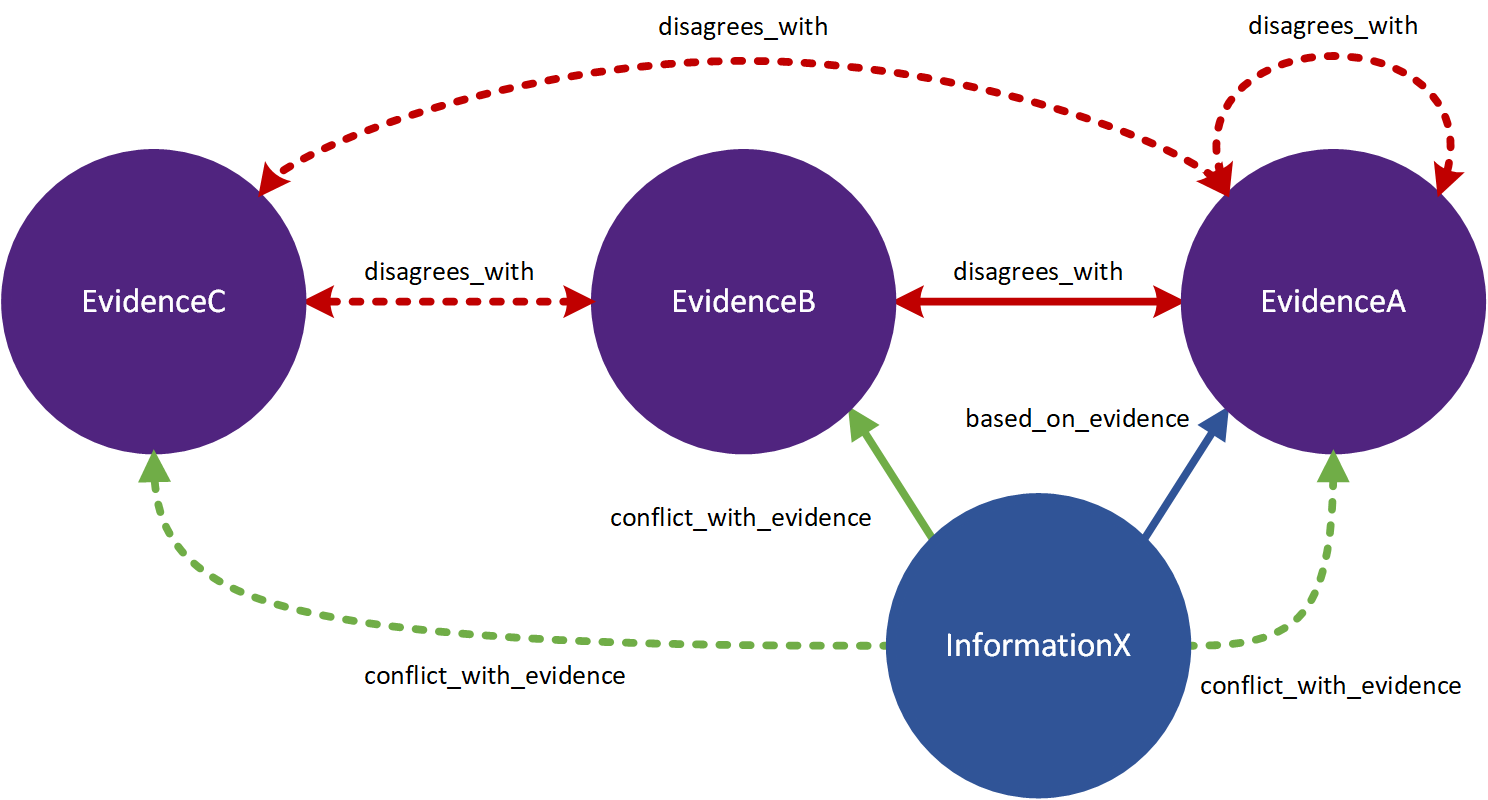
\includegraphics[width=13cm]{../../Images/Conflict_Transitive.png}
  \caption{The transitive characteristic of $disagrees\_with$ causes an inconsistent ontology. The reasoner infers the dotted lines based on the super property figure \ref{fig:conflict_inferred} presents.}
  \label{fig:conflict_transitive}
\end{figure}

\paragraph{Generic ontology design pattern}
Code sample \ref{GODP_CONF_LEV} presents the described solution into GDOL. We take the $Reproducibility\_Basic$ pattern and add the $disagrees\_with$ and $conflict\_with\_evidence$ object properties.

\begin{lstlisting}[float,language=GDOL,caption={The GDOL code that extends the reproducibility pattern and results in the conflict pattern. We take the $Reproducibility\_Basic$ pattern and add the $disagrees\_with$ and $conflict\_with\_evidence$ object properties.},label={GODP_CONF_LEV}][H]
ontology Conflict = Reproducibility_Basic then
  ObjectProperty: disagrees_with Domain: Evidence Range: Evidence Characteristics: Symmetric, Irreflexive
  ObjectProperty: conflict_with_evidence SubPropertyChain: based_on_evidence o disagrees_with SubPropertyOf: conflict_with_evidence
end
\end{lstlisting}

\paragraph{Constraints}
The conflict pattern requires the definition of a conflict level. Conflict reduces the reliability of the information and evidence. Therefore, we do not accept any conflict for our evidence and define the maximum conflict-level as $0$. Any conflict that the constraints detect immediately causes a violation. We use the cardinality constraint $sh:minCount$ for this detection: each individual classified as $In{\f}ormation$ should not have any path (object property) $conflict\_with\_evidence$.

\begin{lstlisting}[float,language=SHACL,caption={The SHACL shapes that detect if there is conflict. },label={SHACL_CONF_LEV}][H]
Used_InformationShape a sh:NodeShape;
	sh:targetClass Used_Information; 
	sh:property [
		sh:path conflict_with_evidence; 
		sh:severity sh:Violation; 
		sh:maxCount 0; 
		sh:message "Conflict detected. Please resolve the conflict or re-consider using this information."; ];
\end{lstlisting}